
\title{ConvNet Lab for DD2427}
\author{
        Miquel Marti Rabadan\\921019-1459\\miquelmr@kth.se
}
\date{\today}

\documentclass[12pt]{article}

\usepackage{graphicx,palatino}

\begin{document}
\maketitle

\section{ConvNet building blocks}
\subsection{Convolution}
\subsubsection{Convolution by a single filter}

\begin{figure}[htbp]
 \centering
 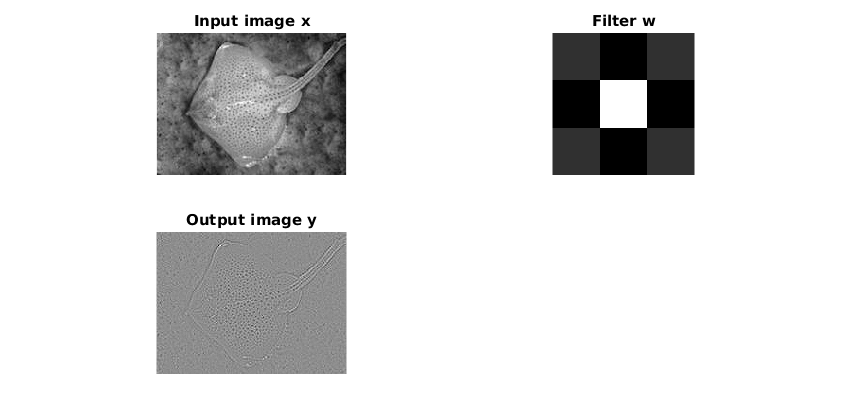
\includegraphics[width=0.8\textwidth]{conv}
 \caption{Convolution with a single filter.}
 \label{fig:q1}
\end{figure}

\paragraph{Question 1: If H x W is the size of the input image, H' x W' the size of the filter, what is the size H'' x W'' of the output image? Why?}
Different strategies apply giving different results. If only using the valid part of the image, no zero-padding, the resulting size is H''=H-(H'-1) x W''=W-(W'-1) because the value cannot be computed in the edges as there is no value to use when applying the kernel.
\paragraph{Question 2: The filter w given above is a discretized Laplacian operator. Which type of visual structures (corners, bars, ...) do you think may excite this filter the most?}
It will excite the most the edges, colour level discontinuities in the image.
\paragraph{Task 1: Suggest a way that you can make the output size be same as the input image size? Apply your suggestion using vl\_nnconv.}
Using zero padding around the image so the image edges have values around it that allow to compute the operation. y = vl\_nnconv(x, w, [],'Pad',1) ; Adds padding around the pixels of the input image before operating.

\subsubsection{Convolution by a filter bank}
\paragraph{Question 3: What is the number of feature channels K in this example? Why?} The number of feature channels is 3, one for each of the filters in the filter bank.
\paragraph{Task 2: Run the code above and visualize the individual feature channels in the tensor y by using the provided function showFeatureChannels(). Do the channel responses make sense given the
filter used to generate them?} Feature channel 1 shows the same result as in previous section. Feature channel 2 enhances more the vertical edges while feature channel 3 the horizontal.
\paragraph{Task 3: Implement the Sobel kernel as another channel and compare the results. Do you see any difference? Explain.} The difference is difficult to see but computing it and showing the result shows that there is a difference, mainly in the center of the edges which seem to have higher value.
\paragraph{Question 4: If the input tensor x has C feature channels, what size should be the third dimension of w?} It should have size C, one slice for each channel.
\paragraph{Question 5: In the code above, the command wbank = cat(4, w1, w2, w3) concatenates the tensors w1, w2, and w3 along the fourth dimension. Why are we interested in filters with 3 dimensions?} Because as said in the previous question each filter should have as many 2D arrays as channels in the input tensor.
\subsubsection{Convolving a batch of images}
\paragraph{Task 4: Run the code above and visualize the result. Convince yourself that each filter is applied to each image. Explain the procedure you used to check this?} First using \texttt{size(y)} gives: 148x198x5x2, being 5 the number of channels and 2 the number of images that were concatenated in the 4th dimension of the input tensor x. Using \texttt{showFeatureChannels(y(:,:,:,1)} the resulting feature channels of the first image are shown, same can be done for the second. See Figure \ref{fig:113}.

\paragraph{Question 6: Why are we interested in working on (mini) batches of images instead of single images? Give all the reasons that you know.} We are interested in doing that because we can re-use a filter bank and apply it at the same time against a bigger number of images. 
\begin{figure}[htbp]
 \centering
 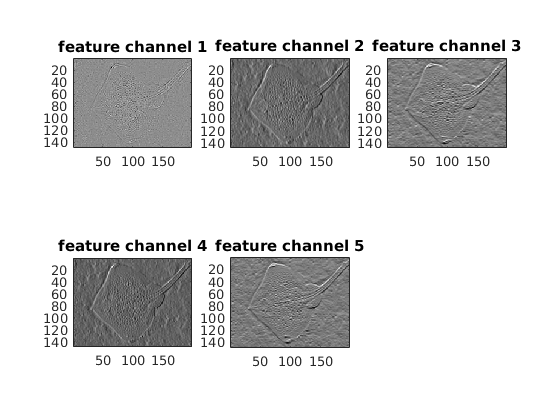
\includegraphics[width=0.8\textwidth]{113a}
 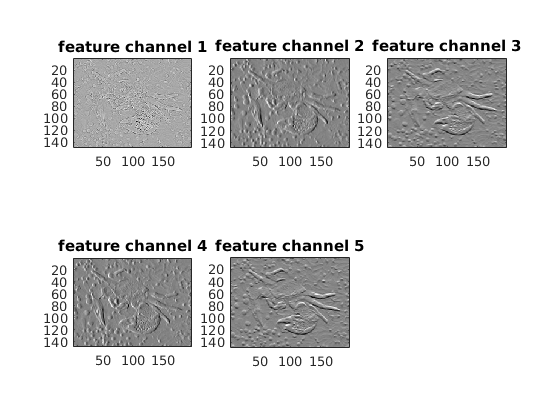
\includegraphics[width=0.8\textwidth]{113b}
 \caption{Convolution of batches with filter bank.}
 \label{fig:113}
\end{figure}

\subsection{Non-linear activation: ReLU}
\paragraph{Question 7: What happens if all layers are linear?}That they can only represent linear functions as the sum of linear layers is linear.
\paragraph{Task 5: Run this code and visualize images x, y, and z.} The result can be seen in Figure \ref{fig:121}.

\begin{figure}[htbp]
 \centering
 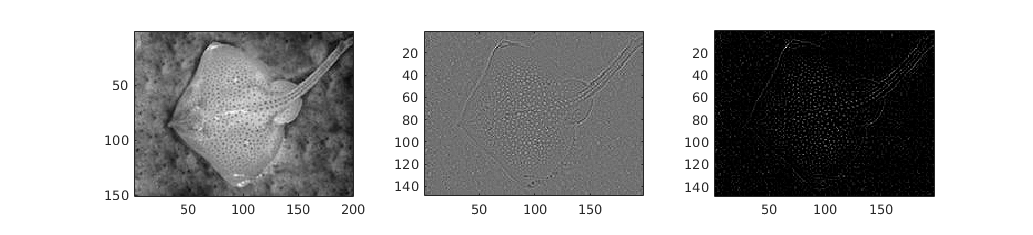
\includegraphics[width=\textwidth]{121}
 \caption{Left to right: original, filtered image and through non-linearity.}
 \label{fig:121}
\end{figure}
\paragraph{Question 8: Which kind of image structures are preferred by this filter?} Isolated dots with high value.
\paragraph{Question 9: Why did we negate the Laplacian?} So that opposite to the first time it was used dots have high value and edges low and when the non-linear ReLU is applied only the dots survive, everything else has the same value of 0.
\paragraph{Task 6: Repeat the same procedure and replace the non-linearity function with sigmoid and tanh. Explain the differences you see between the results of these three operations. Particularly, how is the distribution of the values out of these three activation functions different?} Figure \ref{fig:121b} shwos the different activation functions after the negated Laplacian filter is applied. The tanh and the sigmoid functions behave in a similar way, compressing to high and low values, while the ReLU sets all values below 0 to that value. Compressing only the lower end.

\begin{figure}[htbp]
 \centering
 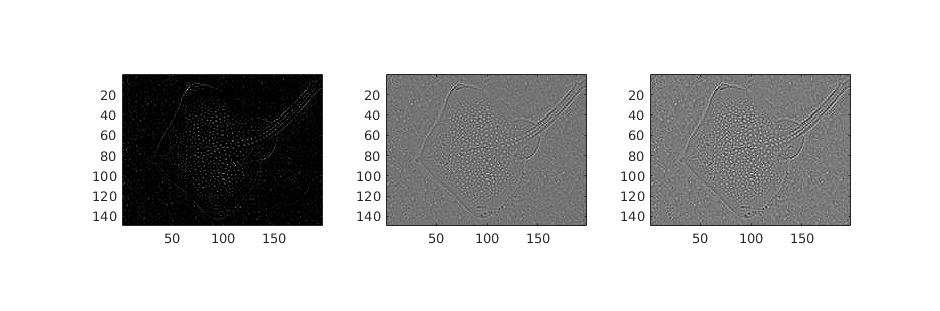
\includegraphics[width=\textwidth]{121b}
 \caption{Different activation functions. Left to right: ReLU, sigmoid and tanh.}
 \label{fig:121b}
\end{figure}

\paragraph{Task 7: Run this code and visualize images x, y, and z.} Figure \ref{fig:122} shows the result.
\paragraph{Question 10: Is the response now more selective?} It is as now fewer pixels are over the zero value.

\begin{figure}[htbp]
 \centering
 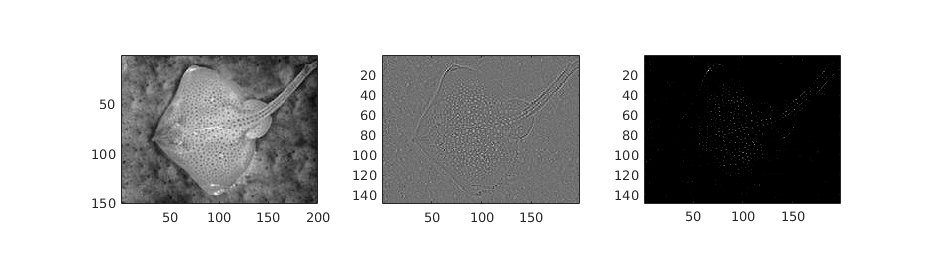
\includegraphics[width=\textwidth]{122}
 \caption{ReLU with bias of -0.2}
 \label{fig:122}
\end{figure}

\paragraph{Task 8: Take a look at the available functionalities provided by MatConvNet.	Find the functionality that can do both max pooling and average pooling. Apply both max and average pooling with a couple of different sizes on both the input image and the output of the convolution. Visualize the results. Discuss the results.} Figure \ref{fig:max} shows the result of applying max and average pooling to the input image and to the output image with different sizes.

\begin{figure}[htbp]
 \centering
 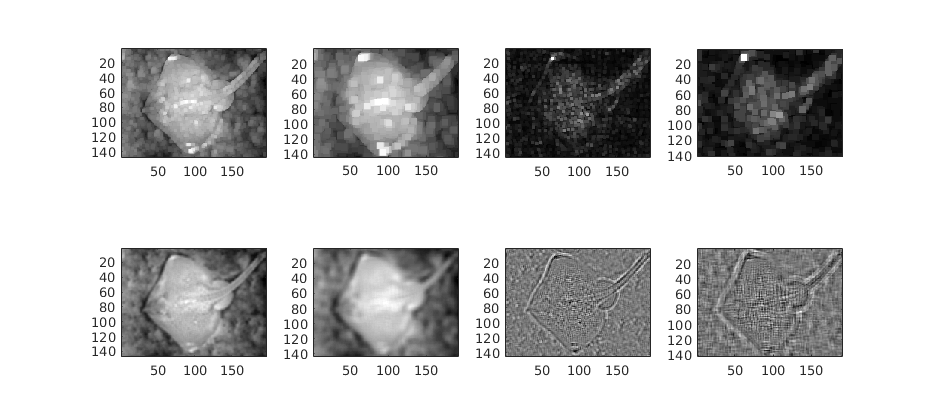
\includegraphics[width=\textwidth]{max}
 \caption{Max (top) and average (bottom) pooling examples.}
 \label{fig:max}
\end{figure}

\section{Backpropagation}
\paragraph{Question 10: The output derivatives have the same size as the parameters in the network. Why?} They have the same size because...
\end{document}


